\chapter{Sprints}
\settocdepth{chapter}
\label{Sprints}

\section{Planning}
\begin{figure}[t]
\centering
    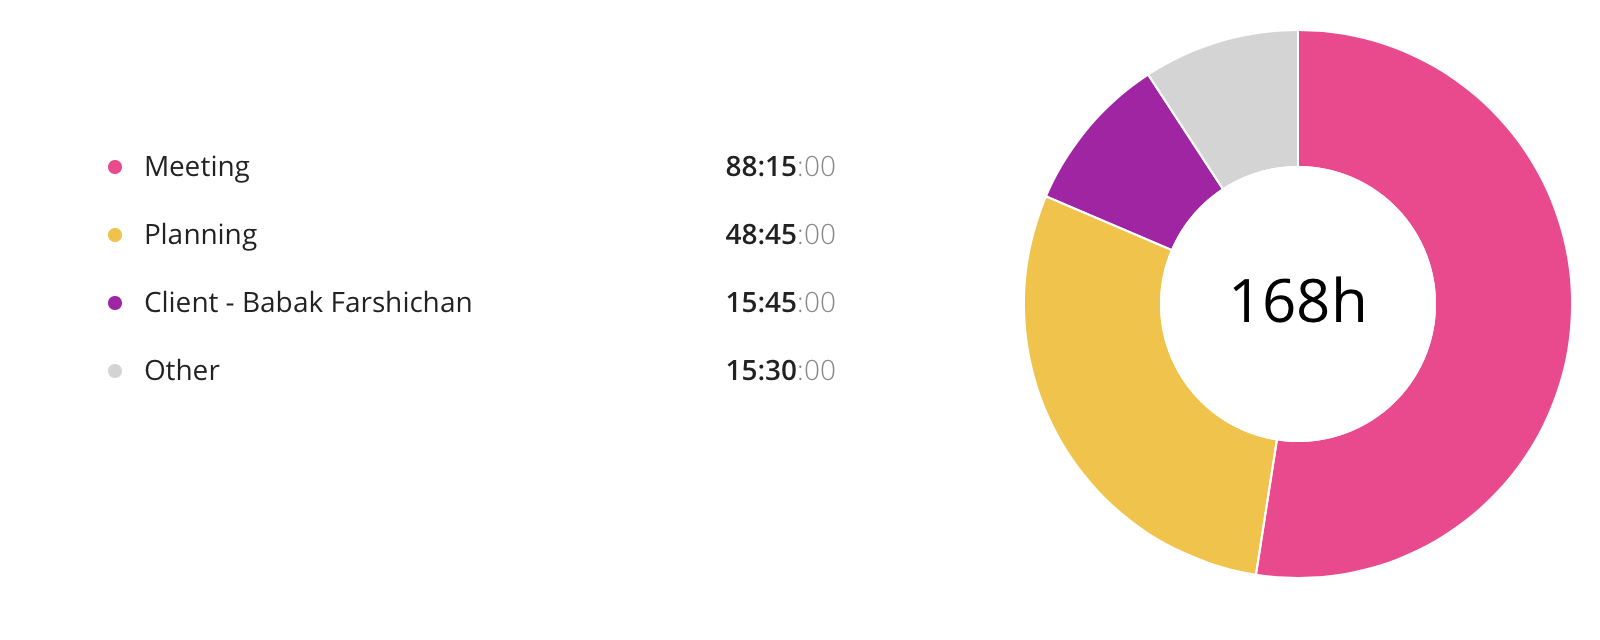
\includegraphics[width=0.6\textwidth]{fig/planning-and-research-diagram}
\caption{Planning - Distributed Time}
\end{figure}

\section{Sprint 0}
The groups drew the design draft as a paper prototype (see section \ref{ss:paper_prototype}), and the group performed a demonstration to the customer. He was satisfied with the idea, and it created a great discussion about how the group should continue working.

The group was satisfied with their own efforts during the sprint. Heaps of work was accomplished, and everyone was motivated to keep working next sprint.
    
The group agreed that they should be more effective during their work sessions, aiming on accomplishing more. To achieve this it is important that everyone takes responsibility of keeping the group on track, and  make sure everyone are concentrated on the tasks at hand.

See fig. \ref{sprint0_burndown} and \ref{sprint0_diagram} for the work distribution during the sprint.

\begin{figure}[ht]
\centering
    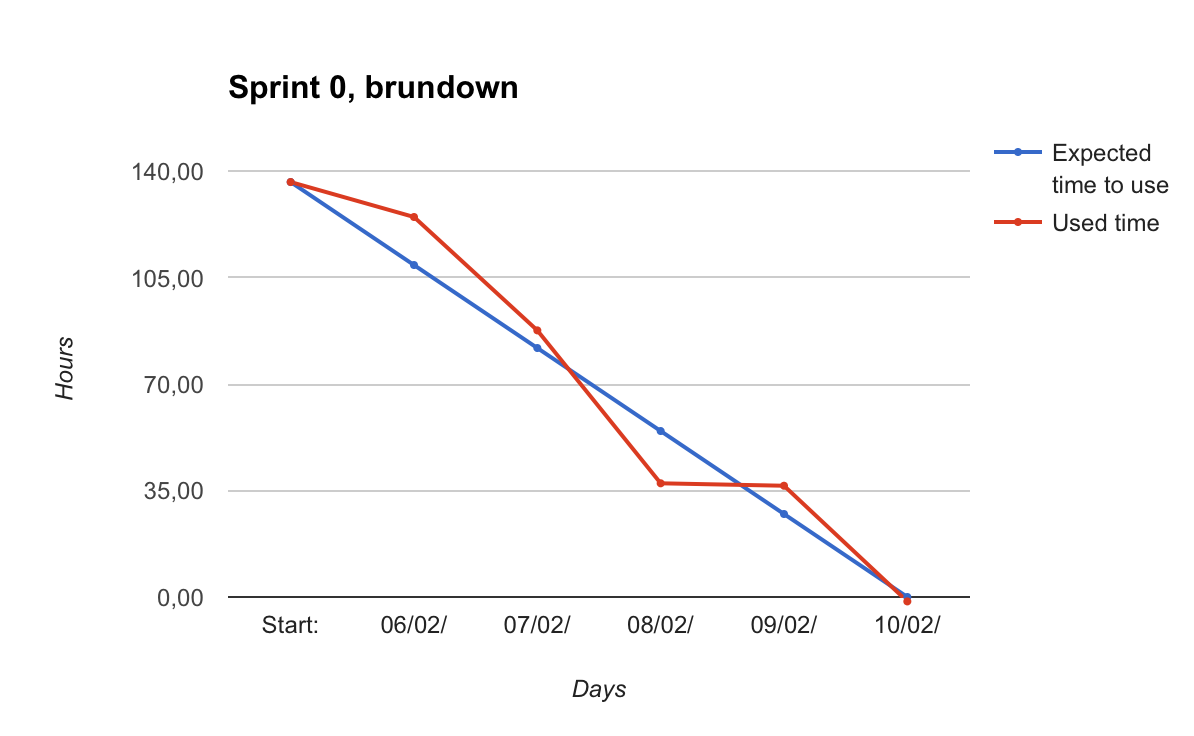
\includegraphics[width=0.8\textwidth]{fig/sprint0}
\caption{Sprint 0 - Burndown} 
\label{sprint0_burndown}
\end{figure}

\begin{figure}[ht]
\centering
    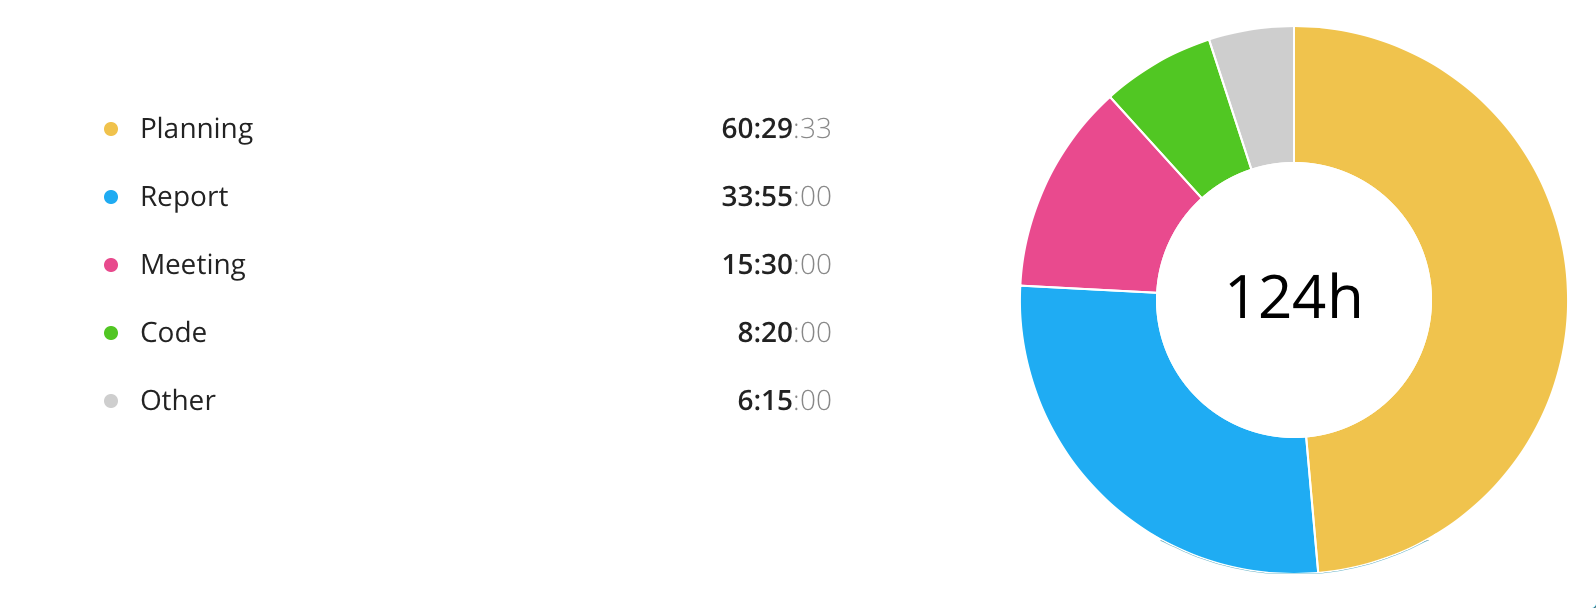
\includegraphics[width=0.8\textwidth]{fig/sprint0-diagram}
\caption{Sprint 0 - Distributed Time}
\label{sprint0_diagram}
\end{figure}

\section{Sprint 1}
\label{Sprints-sprint1}
Two problems were encountered during this sprint. Firstly, one group member asked for five days off to travel. The group concluded this was very inconvenient this early on in the development process, and all resources were necessary to complete the sprint goal. To manage such problems in the future, the group updated their risk analysis (see section \ref{updated_risk_analysis}). 

The second problem encountered was a misunderstanding between the group and the customer, specifically the definition of "proof of concept". The group thought that the web portal should include all functionalities, as a system ready for production. The customer, on the other hand, wanted the design of the concept fully completed but not necessarily a fully functional web portal. The group resolved this with a new meeting with customer and a technical manager at Sintef Digital, and discussed the groups possibilities (see section \ref{webhotel_vs_webserver}). The problem was solved during the meeting.

Because of the misunderstanding with the customer, the group had a discussion on how much time to actually spend on the project. After resolving the misunderstanding with customer, the group concluded that the already scheduled hours should remain.

See fig. \ref{sprint1_burndown} and \ref{sprint1_diagram} for the work distribution during the sprint.

\begin{figure}[ht]
\centering
    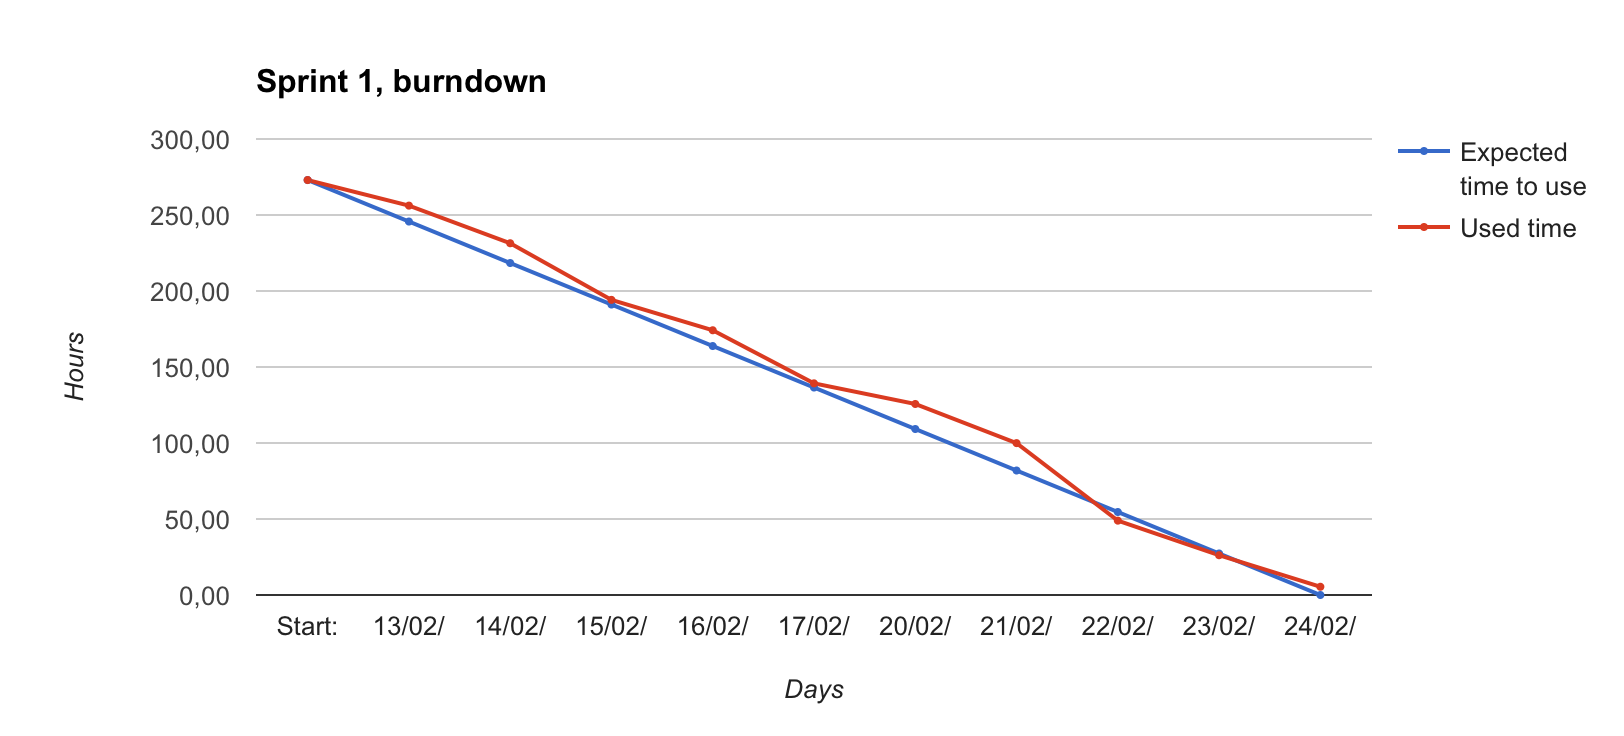
\includegraphics[width=0.8\textwidth]{fig/sprint1}
\caption{Sprint 1 - Burndown}
\label{sprint1_burndown}
\end{figure}

\begin{figure}[ht]
\centering
    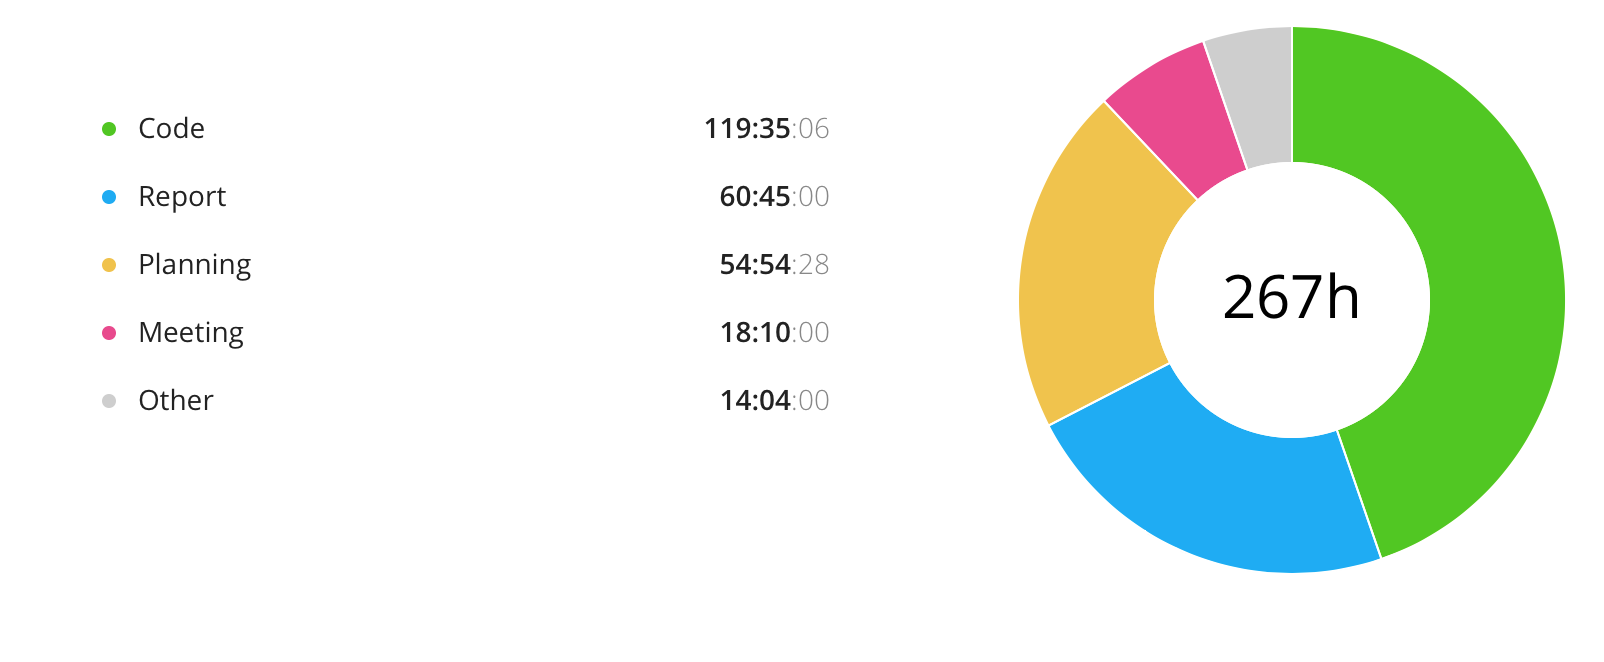
\includegraphics[width=0.8\textwidth]{fig/sprint1-diagram}
\caption{Sprint 1 - Distributed Time}
\label{sprint1_diagram}
\end{figure}

\section{Web-Hotel vs. Web-Server}
\label{webhotel_vs_webserver}
The options for the web portal platform were using a web-hotel or a web-server. The group had several meetings with the customer regarding this decision. The customer primarily wanted to use a web-hotel as hosting service and platform. The group proposed a web-server, rather than dealing with the constraints of using a web-hotel. 

The group suggested to use web-server because it allows for developing the graphical user interface faster and easier by allowing usage of libraries and frameworks, which a web-hotel does not. By utilizing the integrated functionalities offered by libraries and frameworks, time and resources would be more efficiently allocated, as the group would not have to spend time writing this. 

Security is also higher in terms of getting access to the web resources. 
This is because a web-server does not use shared resources. If the web portal was hosted through a web-hotel, the security of the page and its information would only be as safe as the least secure web-page which use the same shared resource. Hosting on a web-server would provide more security for the users of the web portal, and since the application potentially holds sensitive information about the users, security is not to be taken for granted. 

Both web-hotel and web-server could be used as a platform for the web portal. The usage of web-server would make development easier, and allow usage of the best suitable technology for the given task. The group was in a meeting with the customer and an outside developer to present the usage of web-hotel vs. web-server. The group emphasized that the usage of a web-server was a suggestion, and that it was up to the customer to make the final decision. Subsequently, the customer decided to use a web-server, following the group's desire.

\section{Sprint 2}
\label{Sprints-sprint2}
The group experienced couple of problems during this sprint. Firstly, the group came across problems trying to implement the possibility to filter the activities. Initially the group had chosen to use flux, to manage the data flow in the application \cite{flux}. With further research and attempts trying to implement the flux pattern, the group realized it would not be sufficient in this project, as the application was required to support asynchronous actions. Midway in the sprint the group decided to use Redux (see \ref{redux}). To solve this issue the group was required to complete further research on how this should be implemented, this consumed more of the sprint than first expected.

During sprint 1 a set of milestones were defined and arranged after priority, which the group used to define the sprint backlogs. Midway in sprint 2 the customer arouse the desire for one of the final milestones, \textit{"first version of release up and running on server"}, to be completed. To fulfill the customer's desire the group highly prioritized this milestone, which induced difficulties completing the original issues in the sprint backlog. To encounter this issue the group decided to re-prioritize the backlog subsequently after the request from the customer. Moving the milestone at hand to sprint 2 and relocate the milestone "Sign up for activity" to sprint 3. 

Even tough the group encountered a couple of problems, the group was happy with what they had managed to accomplish. These problems affected what was included in the sprint backlog, and subsequently the sprint goal. Still a lot of functionality was implemented and the group worked very well during this period. As an improvement to the upcoming sprints the group decided to become better at focusing on the issues in the sprint backlog.

See fig. \ref{sprint2_burndown} and \ref{sprint2_diagram} for the work distribution during the sprint.

\begin{figure}[ht]
\centering
    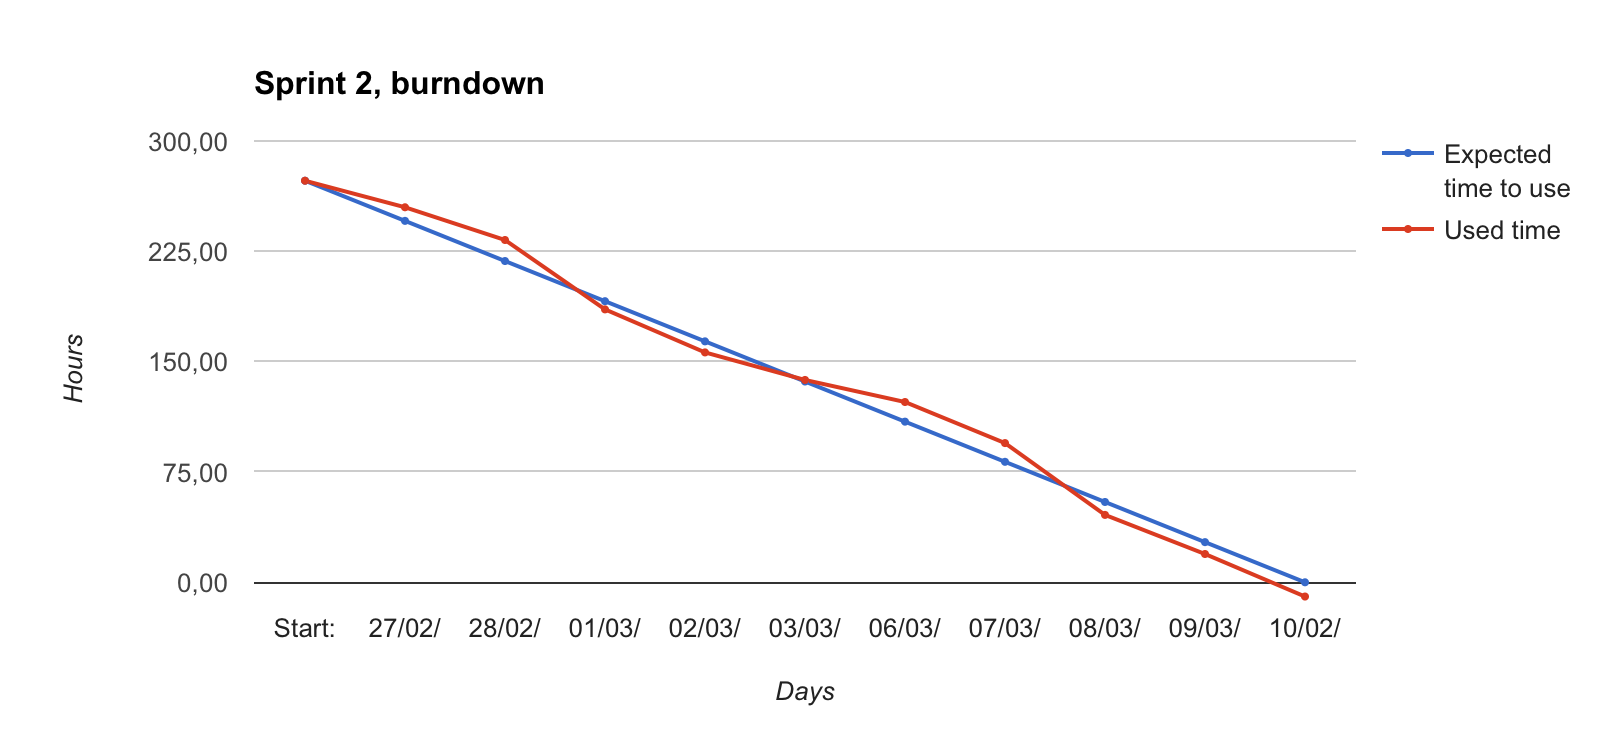
\includegraphics[width=0.8\textwidth]{fig/sprint2}
\caption{Sprint 2 - Burndown}
\label{sprint2_burndown}
\end{figure}

\begin{figure}[ht]
\centering
    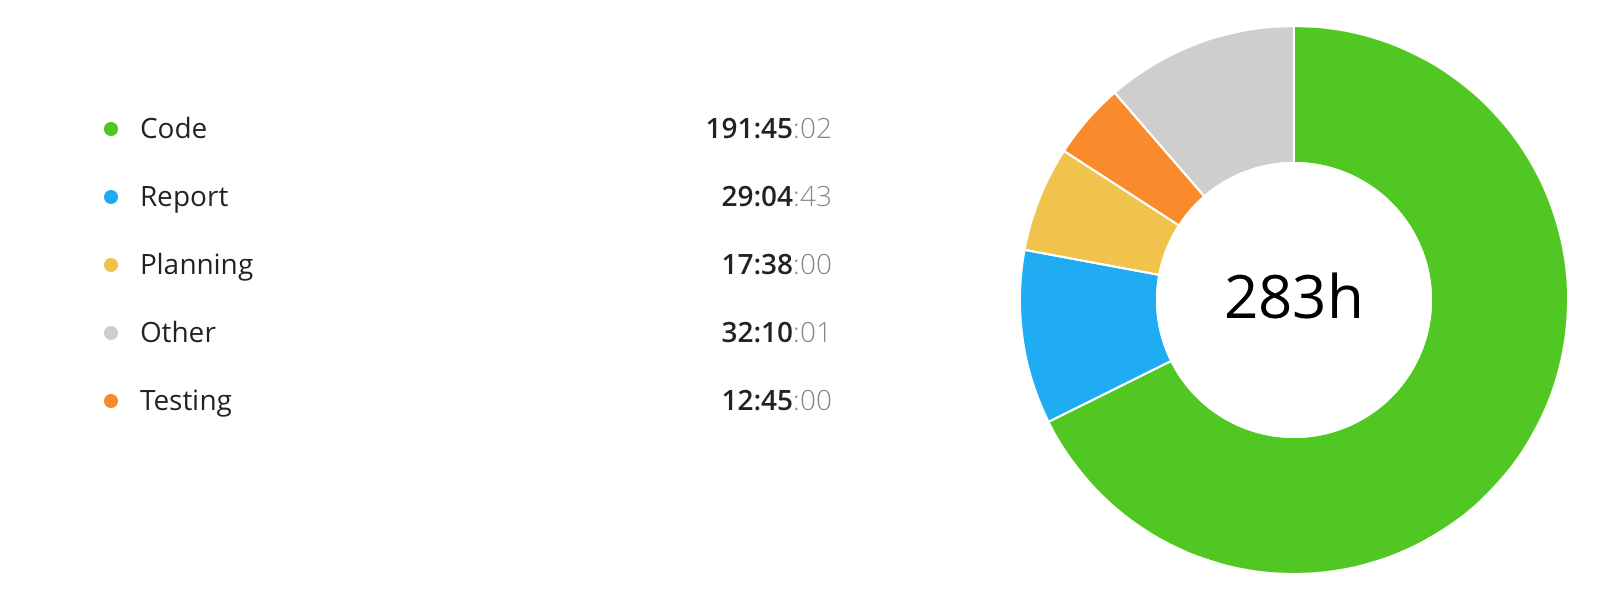
\includegraphics[width=0.8\textwidth]{fig/sprint2-diagram}
\caption{Sprint 2 - Distributed Time}
\label{sprint2_diagram}
\end{figure}

\section{Sprint 4}
\label{Sprints-sprint4}
During the sprint planning, the group went through the product backlog once more and prioritized and re-estimated the workload. The group had previously decided that sprint four was the last sprint where the group could implement new features (see section \ref{s:sprints}). The last couple of weeks of the project should be used to clean up code, fix bugs and focus on documentation. 

The group discussed adding a new feature, robots.txt. Robots.txt, is used to inform web robots not to index any images or other static information. The feature was agreed upon, because of its low cost of implementation and its privacy boost. 

The first thing that was finalized in sprint 4, was the easy installation and guide. The rest of the sprint went really well and there were none problems or other issues during the sprint, all features was implemented.

The group conducted a focus-group test with providers and possible system maintainers (see \ref{before_focus_group_with_providers}). Group members Skaugvoll and Norstein, represented and held the test on behalf of the group. The group demonstrated a few possible scenarios and the main concepts. 

See fig. \ref{sprint4_burndown} and \ref{sprint4_diagram} for the work distribution during the sprint.

\begin{figure}[ht]
\centering
    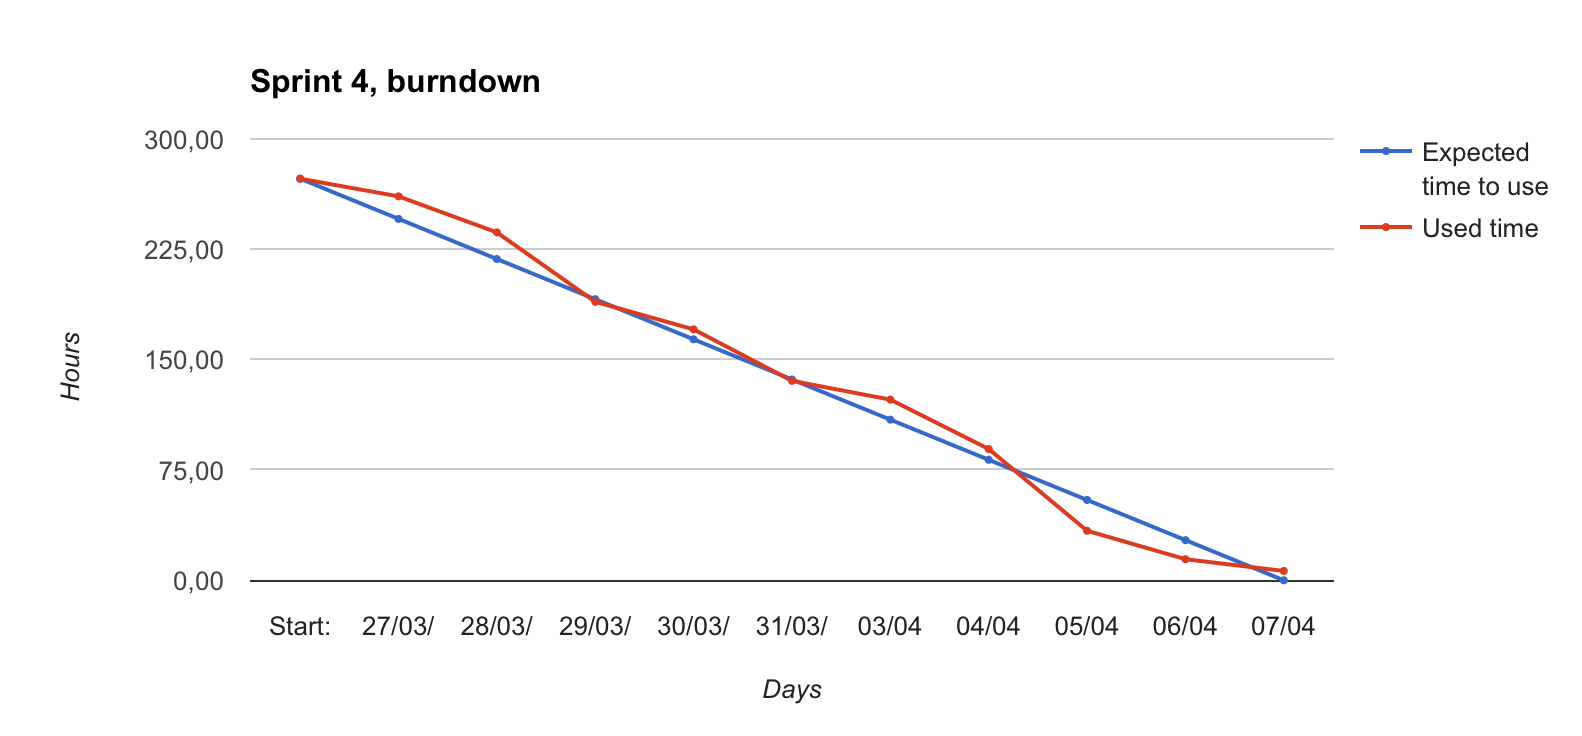
\includegraphics[width=0.8\textwidth]{fig/sprint4}
\caption{Sprint 4 - Burndown}
\label{sprint4_burndown}
\end{figure}

\begin{figure}[ht]
\centering
    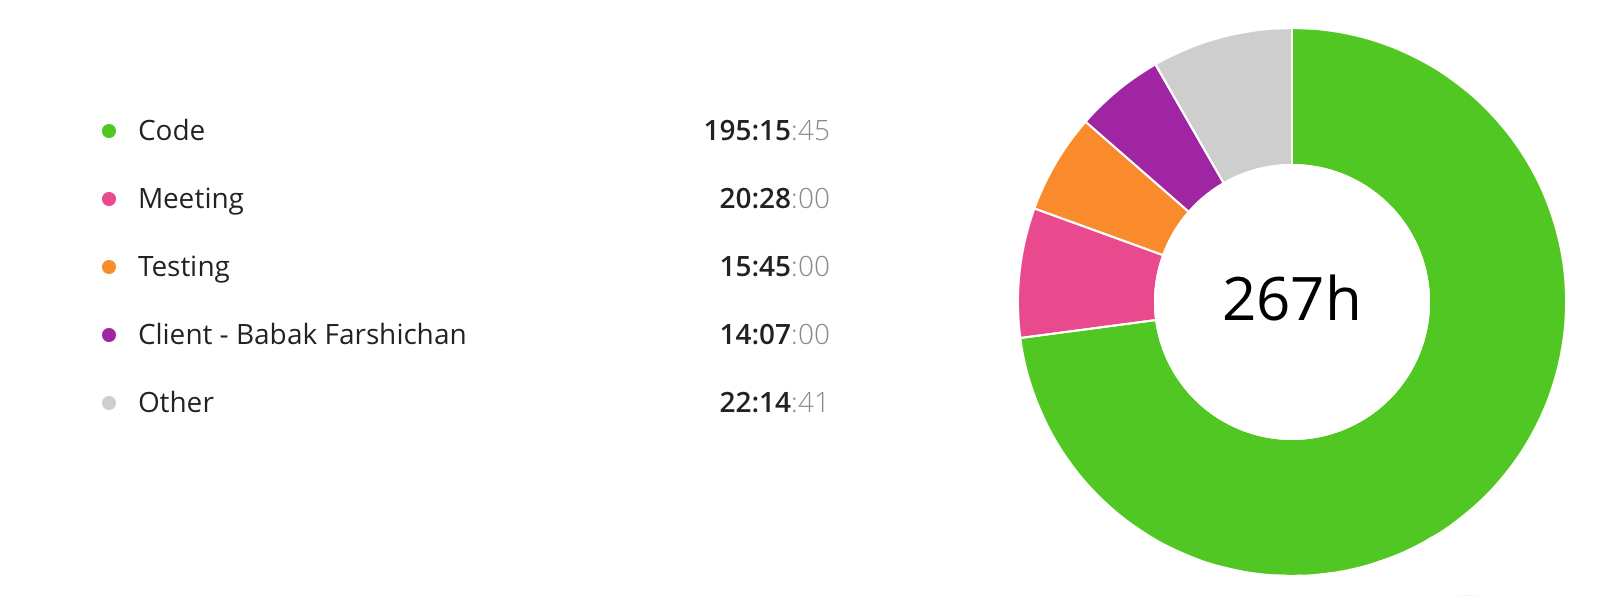
\includegraphics[width=0.8\textwidth]{fig/sprint4-diagram}
\caption{Sprint 4 - Distributed Time}
\label{sprint4_diagram}
\end{figure}

\section{Sprint 5}
\label{Sprints-sprint5}

The sprint ended with structuring and cleaning of the code. The information on GitHub was also updated so that the product could be delivered to the customer as complete and documented as possible.

See fig. \ref{sprint5_burndown} and \ref{sprint5_diagram} for the work distribution during the sprint.

\begin{figure}[ht]
\centering
    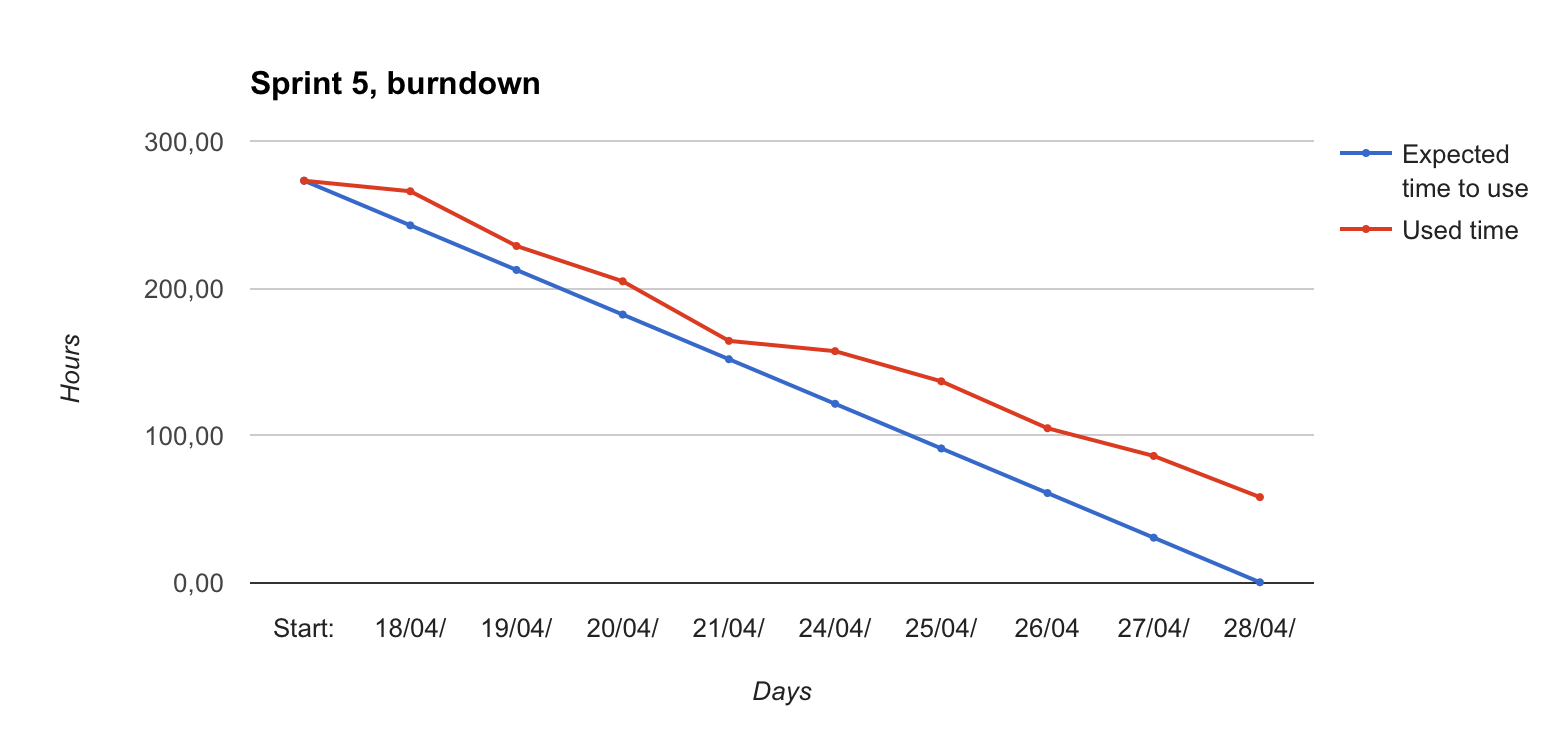
\includegraphics[width=0.8\textwidth]{fig/sprint5}
\caption{Sprint 5 - Burndown}
\label{sprint5_burndown}
\end{figure}

\begin{figure}[ht]
\centering
    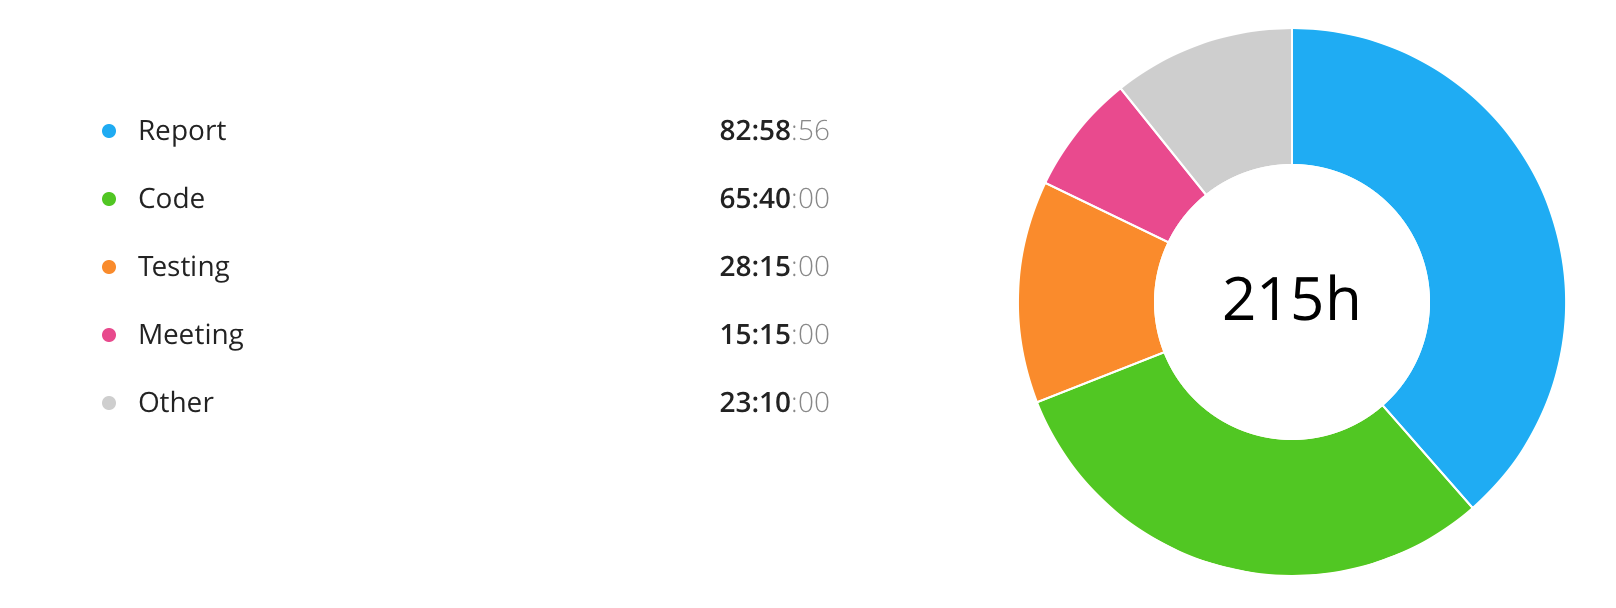
\includegraphics[width=0.8\textwidth]{fig/sprint5-diagram}
\caption{Sprint 5 - Distributed Time}
\label{sprint5_diagram}
\end{figure}

\section{Sprint 6}
\label{Sprints-sprint6}

See fig. \ref{sprint6_burndown} and \ref{sprint6_diagram} for the work distribution during the sprint. 

\begin{figure}[ht]
\centering
    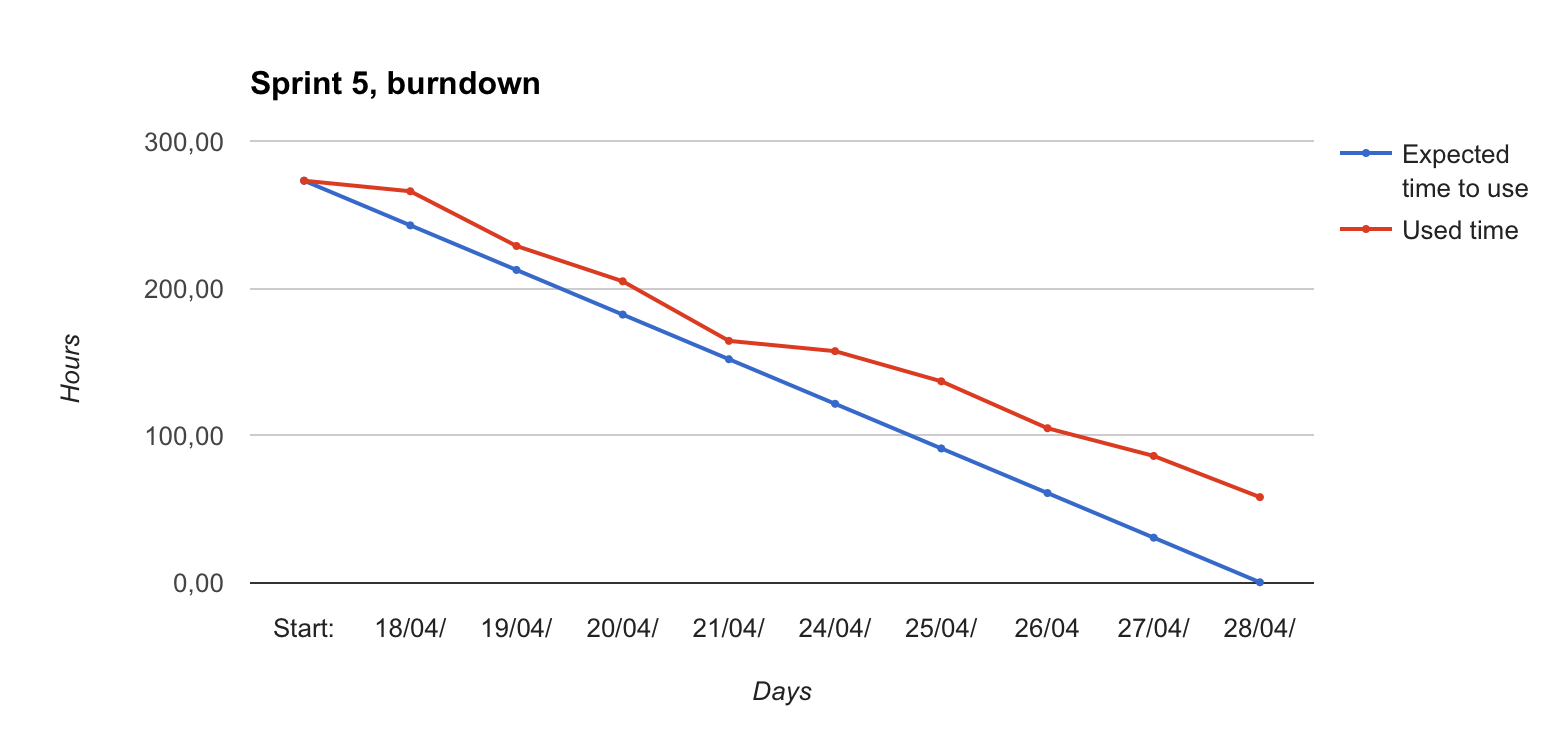
\includegraphics[width=0.8\textwidth]{fig/sprint5}
\caption{Sprint 6 - Burndown}
\label{sprint6_burndown}
\end{figure}

\begin{figure}[ht]
\centering
    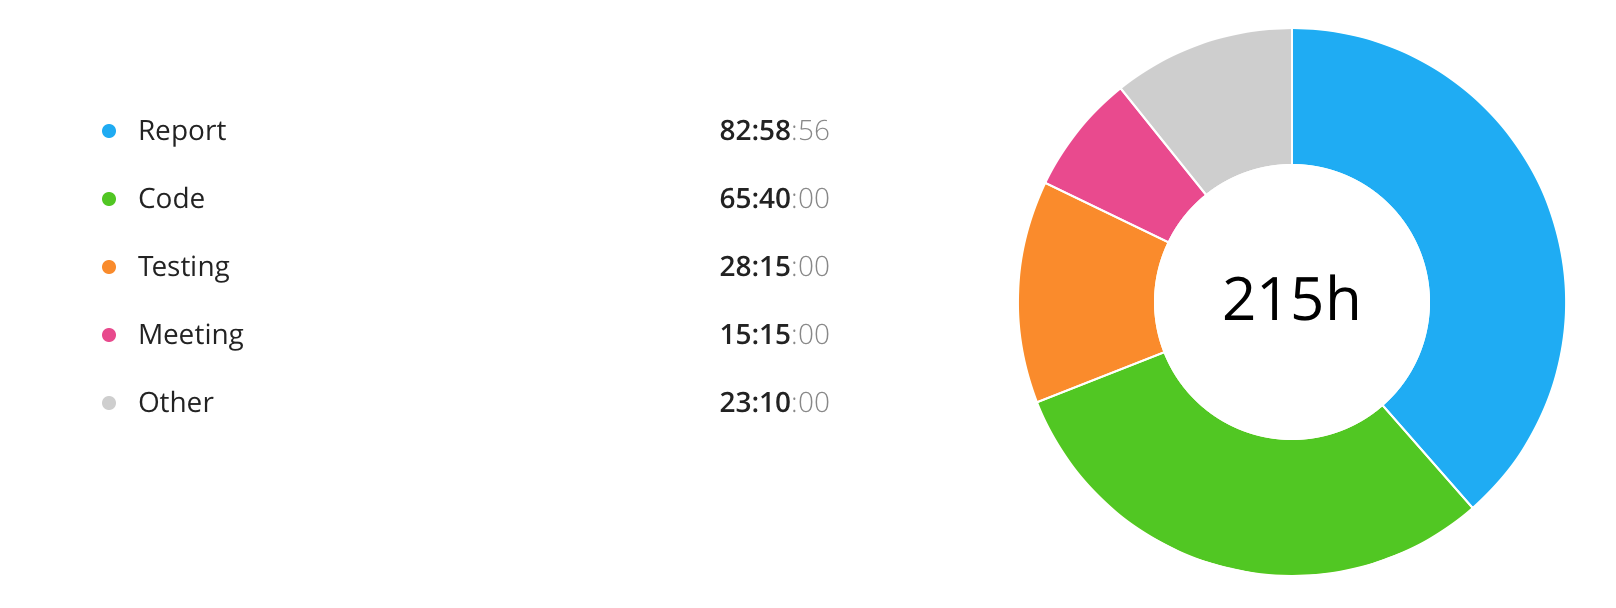
\includegraphics[width=0.8\textwidth]{fig/sprint5-diagram}
\caption{Sprint 6 - Distributed Time}
\label{sprint6_diagram}
\end{figure}

See poster, \ref{poster}, that was showed during demonstration day. 

\begin{figure}[ht]
\centering
    
\includegraphics[width=\textwidth]{fig/finalPoster}
\caption{Poster}
\label{poster}
\end{figure}

\clearpage